\chapter{Introduction}


\section{mRNA life cycle}

Transcription is the first step in gene expression in which a premature RNA molecule is made from a gene's DNA template.
In eukaryotes, splicing, adding a 5$'$ cap and poly-A-tail, as well as binding of cap- and RNA-binding proteins yields mature messenger RNAs (mRNAs).
As transcription and translation are compartmentally separated, these mRNAs are then typically exported through nuclear pore complexes, which perforate the nuclear envelope.
Once in the cytoplasm, the acquired protein coat determines the fate of the mRNA \cite{moore_birth_2005}.
One of these fates is translation to produce proteins.
This process involves polysome (multiple ribosomes translating an mRNA) assembly and messenger ribonucleoprotein complex remodeling and can occur immediately or delayed, such as in the case of various developmental transcripts (reviewed in \cite{swinburne_intron_2008}).
If a protein no longer needs to be produced, polysomes might get disassembled.
Based on the interactions of mRNA-binding proteins, mRNAs can now be targeted for degradation (reviewed in \cite{schoenberg_regulation_2012}).
Alternatively, subsets of these mRNAs can be packaged into RNA granules (Figure \ref{fig:introduction}A).
RNA granules are cytoplasmic, membrane-less, and evolutionarily conserved aggregates containing various proteins involved in translation initiation and repression (reviewed in \cite{anderson_rna_2006}).

\begin{figure}[b!]
    \centering
    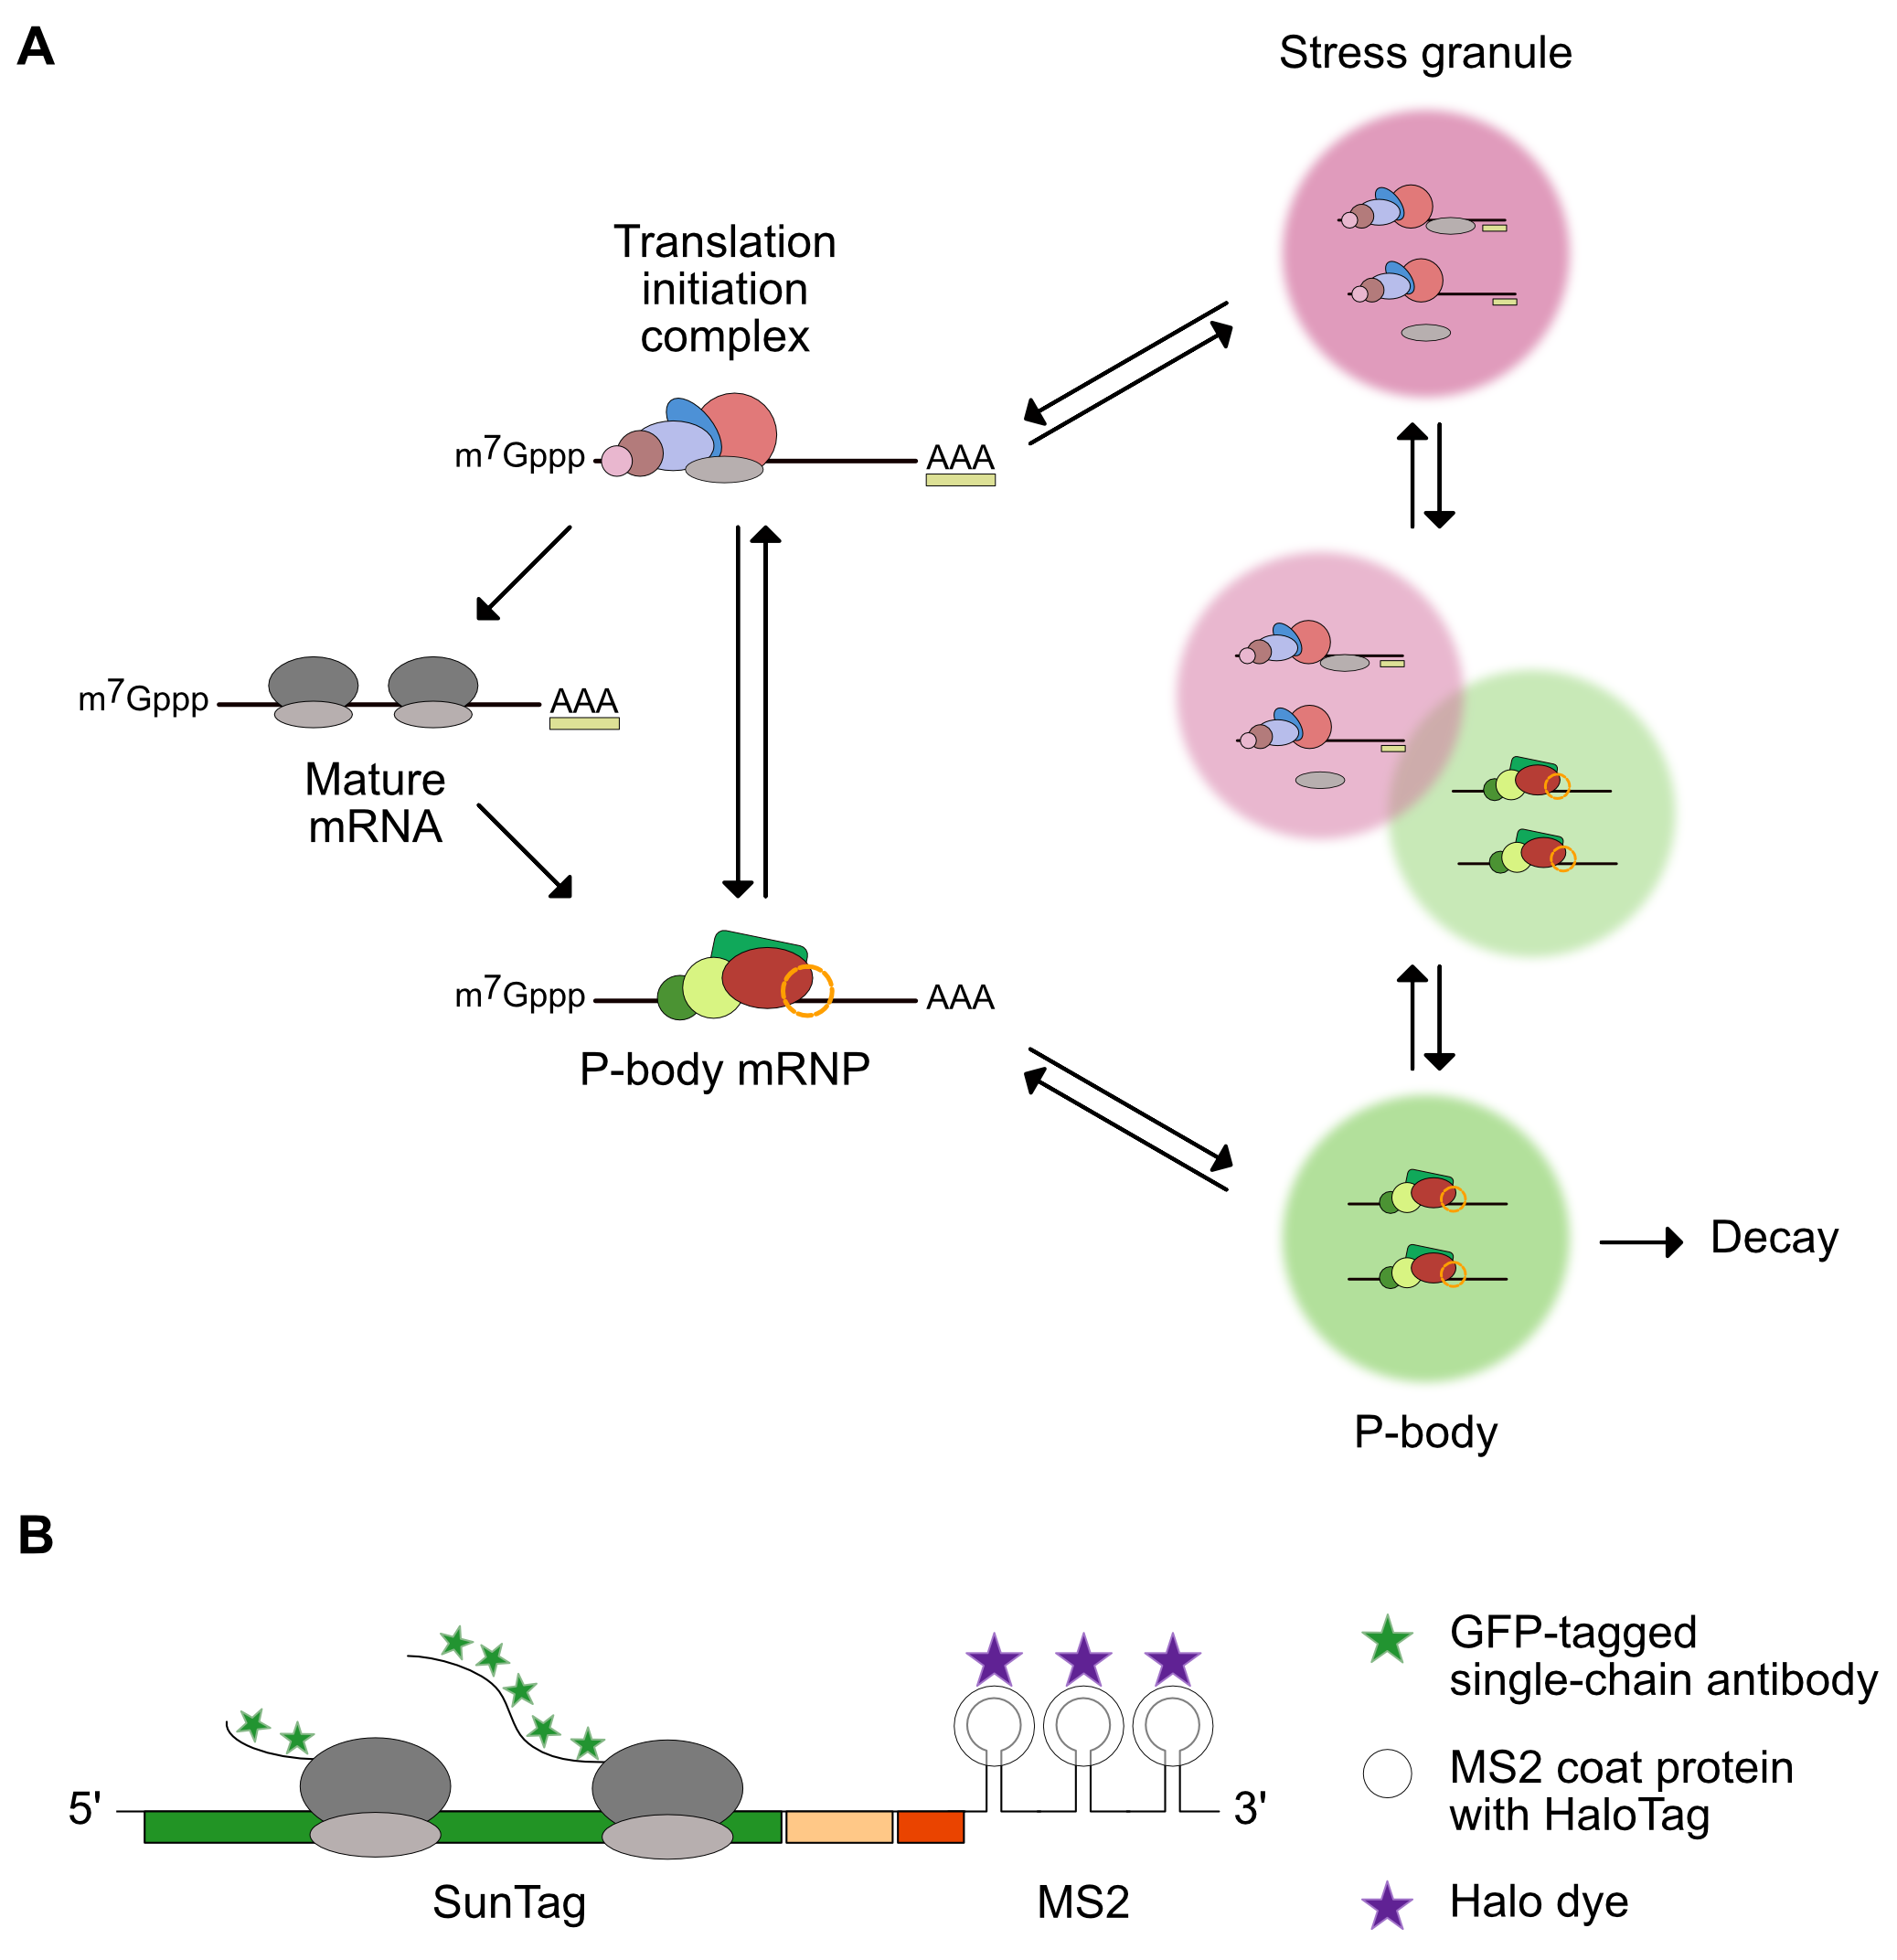
\includegraphics[width=\linewidth]{images/figure1}
    \caption{(Continued on the following page.)}
    \label{fig:introduction}
    \end{figure}
    \addtocounter{figure}{-1}
    \begin{figure} [t!]
    \caption{\textbf{mRNA life cycle and translation site imaging.}
        (A) Overview of a mature, translating mRNAs life cycle.
            Protein components of the translation initiation complex together with their bound
            mRNAs can aggregate into membrane-less organelles termed stress granules.
            A similar type of RNA granule, the P-bodies, have been associated with mRNA
            decay and a different set of proteins.
            Both granules can interact and possibly exchange components.
        (B) Schematic description of SunTag imaging to visualize and quantify
            translational activity on a single-molecule level.
            mRNA building blocks (from left to right): SunTag cassette, \textit{Renilla} luciferase, proteotuner tag, and MS2 stem-loops.
    }
\end{figure}

Stress granules (SGs) are a prominent type of RNA granules that exclusively form under stress.
Cellular stress arises from various external or internal factors and can trigger the integrated stress response pathway.
Typical extrinsic factors range from starvation, infection, hypoxia, the presence of oxidants, and many more.
The largest intrinsic factor is endoplasmic reticulum stress through the accumulation of unfolded or misfolded proteins.
All of these activations converge to the phosphorylation of S52 on the \textalpha\ subunit on eukaryotic translation initiation factor 2 (eIF2\textalpha).
This phosphorylation deactivates eIF2\textalpha\ and inhibits global protein synthesis which can lead to an up-regulation of stress-response genes (reviewed in \cite{pakoszebrucka_integrated_2016}).
Multiple immunofluorescence-based studies have shown that SGs showed an enrichment in initiation factors including eIF2 but not for other translation-related machinery components such as the 60S ribosomal subunit \cite{kimball_mammalian_2003}.
Some proteins found in SGs such as the T-cell intracellular antigen-1 (TIA-1) \cite{kedersha_rna-binding_1999} and Ras GTPase-Activating Protein-Binding Protein 1 (G3BP1) \cite{tourriere_rasgap-associated_2003} have been found to induce SG formation upon overexpression.
The exact nature of SG formation is unknown but various mechanisms from prion-like assembly \cite{gilks_stress_2004, shattuck_prion-like_2019}, maturation of mRNA Processing Bodies (P-bodies) (described below) \cite{buchan_p_2008}, and microtubule involvement have been proposed \cite{ivanov_disruption_2003}.
While SG formation seems to be a conserved phenomenon throughout eukaryotes, their function also remains unclear.
Previous studies have suggested an involvement of SGs in mRNA stability and translational repression (reviewed in \cite{buchan_eukaryotic_2009}).
Furthermore, SG assembly coincides with an accumulation of stalled translation preinitiation complexes in conjunction with polysome disassembly and an increase in uncoated cytoplasmic mRNAs \cite{panas_mechanistic_2016}.
This, along with the observed enrichment of SGs in initiation factors leads to the assumption that SGs exclusively contain translationally repressed mRNAs (reviewed in \cite{thomas_rna_2011}).
However, recent findings from our laboratory have reported that some SG-localized mRNAs can still be translated \cite{mateju_single-molecule_2020}.

A different type of RNA granules, the P-bodies, were originally described as mouse XRN1p (a highly conserved 5$'$-3$'$ exonuclease) foci in the cytoplasm \cite{bashkirov_mouse_1997}.
P-bodies, unlike SGs, are present in unstressed physiology.
However, stress can further increase their formation (reviewed in \cite{parker_p_2007}).
Contrasting SGs, they contain non-overlapping protein components including multiple nucleases that have made them a proposed site of mRNA decay \cite{sheth_decapping_2003}.

Many questions regarding RNA granules, and especially SGs, remain largely unanswered.
For example, their dynamic formation and disintegration, as well as what determines their composition remains unclear.
Several large scale analyses of SGs using spatial proteomics \cite{markmiller_context-dependent_2018, jain_atpase-modulated_2016, youn_high-density_2018} and RNA sequencing \cite{khong_isolation_2018} approaches have given important insights into the content of SGs but not their function.
In a recently published trio of papers \cite{guillen-boixet_rna-induced_2020, sanders_competing_2020, yang_g3bp1_2020} a combination of experiments and computational modeling provided more insights into the formation of SGs.
They hinted at G3BP1 being a key hub in the SG protein interaction network playing a central role during SG formation by RNA-induced conformational changes.
None of these studies, however, gave insights into the biological function that G3BP1 or other SG components exert on single mRNAs.
Recently established single-molecule techniques allow for real-time analyses in live cells.
Compared with extensively used bulk assays, these give a higher spatio-temporal resolution of cellular processes.
In this study, single-molecule imaging techniques will be used to address the effects of the SG-protein G3BP1 on an mRNA's life cycle.

    
\section{Translation site imaging} \label{translation_site_imaging}

The stellar explosion SUperNova (SunTag) imaging approach allows for live cell imaging-based analysis to visualize and quantify translation sites \cite{tanenbaum_protein-tagging_2014}.
The SunTag system relies on three core components: a reporter RNA containing a SunTag cassette and MS2 stem-loops, a green fluorescent protein (GFP)-tagged single-chain antibody (scFv) against GCN4, and an MS2 coat protein fused to a HaloTag (Figure \ref{fig:introduction}B).

The MS2 system has been widely adopted to tag and visualize specific mRNAs.
MS2 stem-loops serve as structural motifs and are recognized by the MS2 bacteriophage capsid RNA-binding protein MS2 (MCP) (reviewed in \cite{george_intracellular_2018}).
Typical MS2 tagging involves the visualization of single mRNAs encoding an array of MS2 stem-loops by an MCP-GFP fusion.
Multiple MS2 stem-loops are used to increase the local concentration of MCP bound fluorescent molecules allowing for significant signal amplification.
Previous studies have used this method to investigate mRNA metabolism by tethering mRNAs to membranes \cite{genz_association_2013}, to proteins \cite{bos_tethered_2016}, or to themselves as shown in a recent optogenetic mRNA clustering approach \cite{kim_optogenetic_2020}.

Currently available standard SunTag cassettes consist of 24 GCN4 epitope repeats that, upon translation and exposure of the GCN4 epitopes, can be recognized and bound by the co-expressed GFP-tagged scFv.
As translation continues, more epitopes get synthesized allowing more scFvs to bind.
This increases the local concentration and thereby brightens the fluorescent signal.
Once translation is terminated, SunTag peptides together with attached scFvs are released from the mRNA causing a decrease in signal intensity.
Degradation of the mature protein is increased due to a proteotuner tag that is located C-terminal of the SunTag cassette and that targets the newly formed protein for proteasomal degradation \cite{azevedo_systematic_2012}.
The MS2 coat protein-HaloTag fusion in conjunction with a soluble Halo dye is used to visualize the MS2 stem loops on the reporter RNA described above.
Taken together, the system allows for accurate tracking of single RNAs and simultaneous quantification of translation.

This study focuses on the understanding of how SGs form and how they function.
Using modified components of the SunTag imaging system, G3BP1 is used as the main antagonist to provide interesting insights into the unknown world of SGs.
G3BP1 will be tethered to a reporter mRNA by fusion to MCP-Halo.
Single-molecule imaging tools including SunTag will be used to investigate the effects of an increased local concentration of SG proteins on mRNA dynamics.
Lastly, an improvement to the existing SunTag system is proposed.
